\begin{question}
\noindent Quadrilateral $Q$ has vertices $A(-3,3)$, $B(-1,3)$, $C(-1,1)$ and $D(-3,0)$.

The line $x=1$ is drawn on the grid below.

\begin{center}
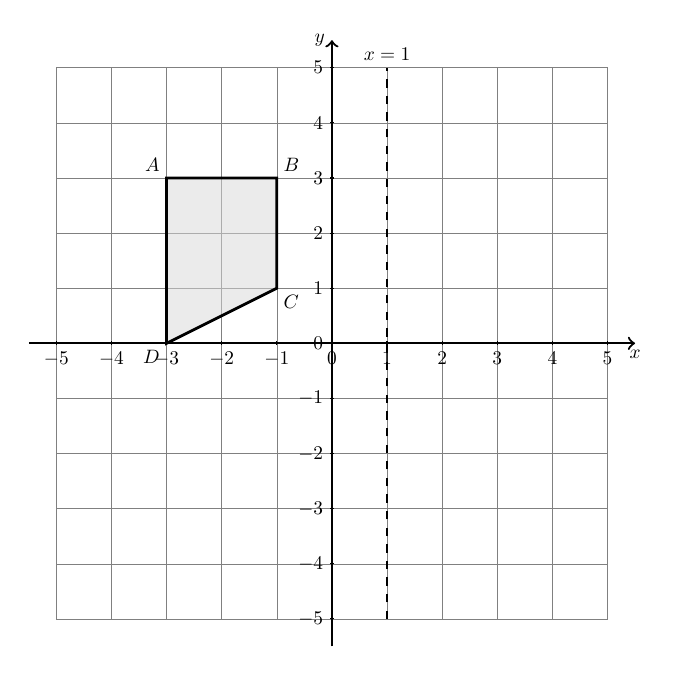
\begin{tikzpicture}[scale=0.7, transform shape]
    \definecolor{borderColour}{HTML}{000000}
    \definecolor{fillColour}{HTML}{D8D8D8}

    \def\axisLimit{5}

    % Draw grid
    \draw[step=1cm,gray,very thin] (-\axisLimit,-\axisLimit) grid (\axisLimit,\axisLimit);

    % Draw axes
    \draw[thick,->] (-\axisLimit-0.5,0) -- (\axisLimit+0.5,0) node[anchor=north] {$x$};
    \draw[thick,->] (0,-\axisLimit-0.5) -- (0,\axisLimit+0.5) node[anchor=east] {$y$};

    \foreach \x in {-\axisLimit,...,\axisLimit}
        \draw (\x cm,1pt) -- (\x cm,-1pt) node[anchor=north] {$\x$};
    \foreach \y in {-\axisLimit,...,\axisLimit}
        \draw (1pt,\y cm) -- (-1pt,\y cm) node[anchor=east] {$\y$};

    % Draw the mirror line x = 1
    \draw[thick,dashed] (1,-5) -- (1,5) node[anchor=south] {$x=1$};

    % Coordinates of quadrilateral Q
    \coordinate (A) at (-3,3);
    \coordinate (B) at (-1,3);
    \coordinate (C) at (-1,1);
    \coordinate (D) at (-3,0);

    \filldraw[fill=fillColour, draw=borderColour, line width=1pt, fill opacity=0.5] (A) -- (B) -- (C) -- (D) -- cycle;

    \node[above left] at (A) {$A$};
    \node[above right] at (B) {$B$};
    \node[below right] at (C) {$C$};
    \node[below left] at (D) {$D$};

\end{tikzpicture}
\end{center}

\noindent Reflect quadrilateral $Q$ in the line $x=1$.

Write down the coordinates of the image of each vertex.

\vspace{4cm}
\answerlines{4}{2}
\end{question}
